\documentclass[a4paper,12pt]{article} 
\usepackage[T1]{fontenc}              
\usepackage[frenchb]{babel} % césures, titres français
\usepackage[utf8]{inputenc} % encodage
\usepackage[a4paper,left=3cm,right=3cm,top=2cm,bottom=2cm]{geometry} % marges
\usepackage{graphicx} % insertion d'images
\usepackage{rotating}
\usepackage{float} % permet d'utiliser H pour placer un flottant obligatoirement
\usepackage{pdfpages} % inclusion de PDF au sein du document
\usepackage{listings}
\pagestyle{plain} % pied de pages simples

\setlength{\parskip}{1ex plus 0.5ex minus 0.2ex} % espace entre les paragraphes
\setcounter{tocdepth}{2}
\setcounter{secnumdepth}{2}

\lstset{% general command to set parameter(s)
basicstyle=\ttfamily, % print whole listing small
keywordstyle=\color{black}\bfseries\underbar,
% underlined bold black keywords
identifierstyle=, % nothing happens
commentstyle=\color{white}, % white comments
showstringspaces=false,
numbers=left,
language=java,
breaklines=true,
frame=tblr} % no special string spaces

%%%% debut macro %%%%
\makeatletter
\renewcommand\section{\@startsection {section}{1}{\z@}%
                           {-3.5ex \@plus -1ex \@minus -.2ex}%
                           {2.3ex \@plus.2ex}%
                           {\normalfont\Large\bfseries}}
\makeatother
%%%% fin macro %%%%



% Def
\newcommand{\code}[1]{{\lstinline{#1}}}

\begin{document}
\newpage
\title{Web Semantique\\TP1}
\date{}
\author{BRIZAI Olivier\\THORAVAL Maxime}
\maketitle

\newpage
\section{Utilisation du raisonneur}
\subsection{Pizza.owl}
Lorsque nous lançons le raisonneur sur l'ontologie \og Pizza.owl \fg{} fournie, nous pouvons observer un changement de couleur pour deux classes : 
\begin{itemize}
	\item CheeseyVegetableTopping
	\item IceCream
\end{itemize}

\subsubsection{CheeseyVegetableTopping}
Une nouvelle ligne est apparue dans la section \og Equivalent Classes \fg{}, il s'agit de \og Nothing \fg{}, elle aussi colorée en rouge.
Un clique sur \og ? \fg{} nous donne des informations sur les axioms sources des erreurs.


\begin{figure}[H]
	\center
	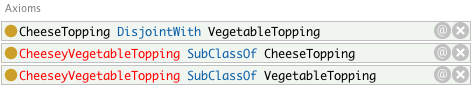
\includegraphics{img/axioms.png}
	\caption{Axioms sources du conflit}
\end{figure}

Dans un premier temps, il est indiqué que les deux classes \og CheeseTopping\fg{} et \og VegetableTopping \fg{} sont disjointes, autrement dit, un objet ne peut être les deux à la fois. Cependant, les lignes suivantes indiquent que la classe \og CheeseyVegetableTopping \fg{} hérite de ces dernières. Il y a ainsi un conflit.


\subsubsection{IceCream}
De la même manière que pour la classe précédente, la sélection de \og ? \fg{} donne des informations sur l'erreur.
\begin{figure}[H]
	\center
	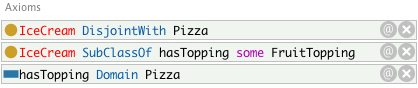
\includegraphics{img/icecream.png}
	\caption{Axioms sources du conflit}
\end{figure}

\og IceCream \fg{}  et \og Pizza \fg{} sont disjointes, \og IceCream \fg{} a au moins une garniture de type \og FruitTopping \fg{}. Il est cependant définit que la propriété \og hasTopping \fg{} a pour domaine \og Pizza \fg{}. Comme vu précédemment, une classe ne peut être à la fois \og IceCream \fg{} et \og Pizza \fg{}. Il y a donc un conflit.


\subsection{Enigme d'Einstein}
L'ontologie crée pour l'énigme d'Einstein démontre l'efficacité et l'utilité du raisonneur. En effet, une fois exécuté, chaque personne est répartie dans la maison appropriée vérifiant les propriétés indiquées dans l'énoncé.

\section{Notre ontologie}
Il s'agit de la représentation des différents types de sièges possibles.
Pour se faire, on considère qu'un siège est découpé en 4 composants : l'assise, le dossier, les accoudoirs et les pieds.
Chacun a sa propre couleur ainsi que son propre matériaux.
De plus, certain peuvent contenir un bourrage (pour être plus moelleux par exemple). On retrouve l'assise, le dossier et les accoudoirs. 

Cette découpe permet de réaliser un grand nombre de combinaison de sièges possible.
Par exemple, une chaise de jardin, il s'agit d'un siège composé d'une assise, d'un dossier, de deux accoudoirs et de quatre pieds, le tout en plastique.\\
La OWLDoc est disponible à l'adresse :
\begin{center}
http://www.ecole.ensicaen.fr/$\sim$thoraval/websemantique/ontologies/doc/
\end{center}

\subsection{Requêtes}
Les requêtes ont été effectuées à partir du site : http://sparql.org/sparql.html.
Notre ontologie est accessible à l'adresse :
\begin{center}
http://www.ecole.ensicaen.fr/$\sim$thoraval/websemantique/ontologies/siege.owl
\end{center}

\subsubsection{Affichage des sièges et de leur support}
\lstset{commentstyle=\textit}
\begin{lstlisting}
PREFIX siege:<http://www.siege.org/ontologies/siege.owl#>
PREFIX rdf:<http://www.w3.org/1999/02/22-rdf-syntax-ns#>
SELECT ?siege ?pied
WHERE { ?siege siege:reposeSur ?pied}
\end{lstlisting}

\begin{figure}[H]
	\begin{center}
		\begin{tabular}{|c|c|} 
			\hline
			\textbf{siege} & \textbf{pied} \\
			\hline
			tabouret12	& piedTab3 \\
			\hline
			tabouret12	& piedTab2 \\
			\hline
			tabouret12	& piedTab1 \\
			\hline
			chaise780 & piedJard4 \\
			\hline
			chaise780 & piedJard3 \\
			\hline
			chaise780 & piedJard2 \\
			\hline
			chaise780 & piedJard1 \\
			\hline
			canape27 & pied2 \\
			\hline
			canape27 & pied1 \\
		\end{tabular}
	\end{center}
\caption{Résultat de la requête}
\end{figure}


\subsubsection{Récupération de toutes les assises de couleur marron}
\begin{lstlisting}
PREFIX siege:<http://www.siege.org/ontologies/siege.owl#>
PREFIX rdf:<http://www.w3.org/1999/02/22-rdf-syntax-ns#>
SELECT ?Assises
WHERE { ?Assises siege:estColoreEn siege:Marron .
        ?Assises rdf:type siege:Assise
	}
\end{lstlisting}

\begin{figure}[H]
	\begin{center}
		\begin{tabular}{|c|} 
			\hline
			\textbf{Assises} \\
			\hline
			assise88 \\
			\hline
			assise87 \\
		\end{tabular}
	\end{center}
\caption{Résultat de la requête}
\end{figure}


\subsubsection{Récupération des sièges, de leur type et de leur nombre de place}
\begin{lstlisting}
PREFIX siege:<http://www.siege.org/ontologies/siege.owl#>
PREFIX rdf:<http://www.w3.org/1999/02/22-rdf-syntax-ns#>
SELECT *
WHERE { ?siege a siege:Siege .
	OPTIONAL {?siege a ?type . 
		FILTER (?type != <http://www.w3.org/2002/07/owl#Thing>) .
		FILTER (?type != siege:Siege)}
	OPTIONAL {?siege siege:nombrePlace ?nbPlaces}
}	
\end{lstlisting}

\begin{figure}[H]
	\begin{center}
		\begin{tabular}{|c|c|c|} 
			\hline
			\textbf{siege} & \textbf{type} & \textbf{nbPlaces} \\
			\hline
			chaise780 & ChaiseDeJardin & 1 \\
			\hline
			canape27 & Canape & 2 \\
			\hline
			tabouret12 & TabouretDeCuisine & 1 \\
			\hline
			canapeSansPlace & CanapeEnTissu & \\
		\end{tabular}
	\end{center}
\caption{Résultat de la requête}
\end{figure}

\end{document}


